\documentclass[10pt, conference, a4paper]{IEEEtran}
\usepackage[utf8]{inputenc}
\usepackage[T5]{fontenc} % Hỗ trợ hiển thị tiếng Việt chuẩn
\usepackage{amsmath,amssymb,amsfonts}
\usepackage{graphicx}
\usepackage{cite}
\usepackage{float} % Thêm package float để cố định vị trí ảnh
\usepackage{tikz}
\usetikzlibrary{shapes.geometric, arrows, positioning}

% Điều chỉnh lại một số nhãn thành tiếng Việt
\renewcommand{\abstractname}{Abstract}
\renewcommand{\figurename}{Hình}
\renewcommand{\refname}{TÀI LIỆU THAM KHẢO}

\begin{document}

\title{Mô Hình Hệ Thống Cảnh Báo Cháy Nổ Và Rò Rỉ Khí Gas Thông Minh}

% Sinh viên thực hiện
\author{
\IEEEauthorblockN{
Trần Thị Huyền Trang (23021924), 
Bùi Đức Dũng (23021777), \\
Lê Mai Việt Hoàng (22022191), 
Nguyễn Duy Phương (23021882)
}
\IEEEauthorblockA{
\textit{University of Engineering and Technology, Vietnam National University}\\
Hanoi, Vietnam
}
}

\maketitle

\begin{abstract}
Trong báo cáo này, chúng tôi nghiên cứu, thiết kế và đề xuất mô hình hệ thống giám sát, cảnh báo cháy nổ và rò rỉ khí gas sử dụng vi điều khiển ESP8266. Hệ thống thu thập dữ liệu trực tiếp từ cảm biến nhiệt độ DHT22, cảm biến khí gas MQ2 và cảm biến phát hiện ngọn lửa. Dựa trên các ngưỡng an toàn được thiết lập, hệ thống tự động đưa ra các kịch bản phản hồi tương ứng như bật còi báo động, mở cửa sổ thông qua động cơ servo, kích hoạt quạt hút khí và hiển thị trạng thái qua cụm đèn LED RGB. Kết quả cho thấy hệ thống hoạt động với tốc độ đáp ứng cao, hỗ trợ tích cực cho các ứng dụng nhà thông minh.
\end{abstract}

\begin{IEEEkeywords}
ESP8266, DHT22, MQ2, cảnh báo cháy, rò rỉ gas, nhà thông minh, IoT.
\end{IEEEkeywords}

\section{GIỚI THIỆU}
Ngày nay, các vấn đề về an toàn phòng cháy chữa cháy và rò rỉ khí độc hại tại các hộ gia đình, cơ sở sản xuất đang nhận được sự quan tâm rất lớn. Việc phát hiện sớm các nguy cơ này có vai trò cực kỳ quan trọng trong việc bảo vệ tính mạng và giảm thiểu thiệt hại tài sản. Hệ thống báo cháy tự động truyền thống thường chỉ có chức năng phát ra âm thanh báo động mà chưa có các cơ chế xử lý tức thời tự động như thông gió hay mở cửa thoát hiểm.

Nhằm giải quyết hạn chế trên, bài báo này đề xuất một giải pháp kết hợp giữa giám sát liên tục và phản hồi tự động dựa trên nền tảng vi điều khiển ESP8266 [1]. Bằng cách tích hợp nhiều cảm biến để đo nhiệt độ, nồng độ khí gas và phát hiện bức xạ từ ngọn lửa [2], hệ thống có khả năng đưa ra các quyết định điều khiển thiết bị ngoại vi ngay lập tức để can thiệp giảm thiểu rủi ro.

Phần còn lại của bài báo được tổ chức như sau: trong phần II, chúng tôi miêu tả chi tiết cấu trúc mô hình đề xuất. Trong phần III, chúng tôi đánh giá hiệu năng của hệ thống qua các kịch bản mô phỏng. Cuối cùng, chúng tôi kết luận bài báo trong phần IV.

\section{MÔ HÌNH HỆ THỐNG}
\subsection{Các linh kiện phần cứng}
Trong mô hình khảo sát, chúng ta xét một hệ thống thu thập số liệu đa chiều sử dụng mạch xử lý trung tâm là ESP8266. Để tăng cường chất lượng phát hiện sự cố, tổ hợp ba cảm biến sau được sử dụng:

\begin{itemize}
    \item \textbf{Cảm biến nhiệt độ DHT22}: Dữ liệu nhiệt độ (ký hiệu là $t$) được đo liên tục để phát hiện sự gia tăng nhiệt độ vượt ngưỡng báo động được thiết lập là $TEMP\_THRESHOLD = 20.0^\circ\text{C}$.
    
    \begin{figure}[H]
    \centerline{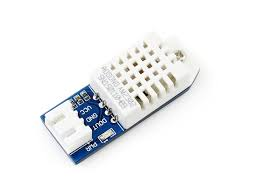
\includegraphics[width=0.45\linewidth]{figures/dht22.jpg}}
    \caption{Cảm biến nhiệt độ DHT22.}
    \label{fig:dht22}
    \end{figure}

    \item \textbf{Cảm biến MQ2}: Chịu trách nhiệm đo nồng độ các loại khí dễ cháy. Tín hiệu đầu vào $gasValue$ được lấy qua bộ chuyển đổi ADC và so sánh với ngưỡng an toàn $GAS\_THRESHOLD = 500$.
    
    \begin{figure}[H]
    \centerline{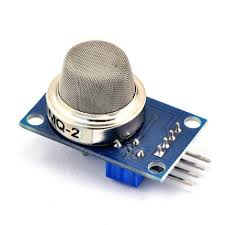
\includegraphics[width=0.45\linewidth]{figures/mq2.jpg}}
    \caption{Cảm biến khí gas MQ2.}
    \label{fig:mq2}
    \end{figure}

    \item \textbf{Cảm biến phát hiện ngọn lửa}: Đưa ra tín hiệu dạng logic (mức LOW khi phát hiện có ngọn lửa) để xác nhận có hỏa hoạn xảy ra.
    
    \begin{figure}[H]
    \centerline{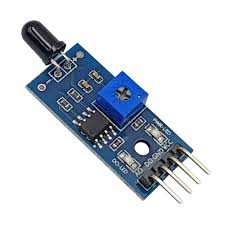
\includegraphics[width=0.45\linewidth]{figures/flame_sensor.jpg}}
    \caption{Cảm biến phát hiện ngọn lửa.}
    \label{fig:flame}
    \end{figure}
\end{itemize}

Về cơ chế xử lý, đầu tiên, xét sự truyền tín hiệu và phản hồi với các bộ chấp hành, chúng ta có thể mô tả hệ thống hoạt động thông qua các ngoại vi sau:

\begin{itemize}
    \item \textbf{Động cơ Servo}: Điều khiển mở cửa sổ (quay $90^\circ$) để thông gió và tạo khoảng không thoát khí.
    
    \begin{figure}[H]
    \centerline{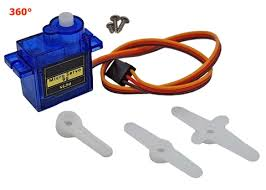
\includegraphics[width=0.45\linewidth]{figures/servo.jpg}}
    \caption{Động cơ Servo.}
    \label{fig:servo}
    \end{figure}

    \item \textbf{Relay (Rơ-le)}: Đóng cắt nguồn điện cho quạt hút, giúp đẩy không khí độc ra khỏi hiện trường.
    
    \begin{figure}[H]
    \centerline{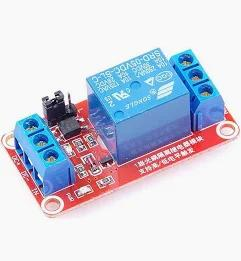
\includegraphics[width=0.45\linewidth]{figures/relay.jpg}}
    \caption{Module Relay.}
    \label{fig:relay}
    \end{figure}

    \item \textbf{Còi báo động (Buzzer)}: Phát âm thanh cảnh báo cường độ cao tại chỗ.
    
    \begin{figure}[H]
    \centerline{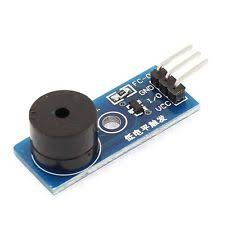
\includegraphics[width=0.45\linewidth]{figures/buzzer.jpg}}
    \caption{Còi báo động (Buzzer).}
    \label{fig:buzzer}
    \end{figure}

    \item \textbf{Đèn LED RGB}: Thay đổi màu sắc (Xanh lá, Vàng, Đỏ) để thông báo mức độ khẩn cấp một cách trực quan.
    
    \begin{figure}[H]
    \centerline{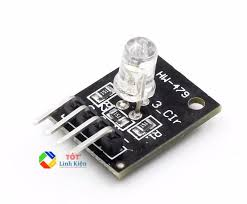
\includegraphics[width=0.45\linewidth]{figures/module_led.jpg}}
    \caption{Module Đèn LED RGB.}
    \label{fig:led}
    \end{figure}
\end{itemize}

Chú ý rằng: toàn bộ hệ thống hoạt động lặp liên tục, chu kỳ lấy mẫu được ấn định là 2000 mili-giây.


\begin{figure*}[!ht]
\centering
\begin{tikzpicture}[
    node distance=1.5cm and 2.5cm,
    sensor/.style={draw, rectangle, minimum width=2.5cm, minimum height=1cm, align=center, fill=blue!10},
    mcu/.style={draw, rectangle, minimum width=3cm, minimum height=6.5cm, align=center, fill=green!10, rounded corners},
    actuator/.style={draw, rectangle, minimum width=2.5cm, minimum height=1cm, align=center, fill=red!10},
    cloud/.style={draw, ellipse, minimum width=3cm, minimum height=1.5cm, align=center, fill=cyan!10},
    arrow/.style={-stealth, thick}
]

% Khối MCU
\node[mcu] (esp) {ESP8266};

% Khối cảm biến (Bên trái)
\node[sensor, left=2cm of esp] (mq2) {Cảm biến \\ MQ2};
\node[sensor, above=0.5cm of mq2] (dht) {Cảm biến \\ DHT22};
\node[sensor, below=0.5cm of mq2] (flame) {Cảm biến \\ Ngọn lửa};

% Khối chấp hành (Bên phải)
\node[actuator, right=2cm of esp, yshift=0.75cm] (relay) {Relay \\ (Quạt hút)};
\node[actuator, above=0.5cm of relay] (servo) {Động cơ \\ Servo};
\node[actuator, right=2cm of esp, yshift=-0.75cm] (buzzer) {Còi báo động};
\node[actuator, below=0.5cm of buzzer] (led) {Đèn LED \\ RGB};

% Khối Cloud (Bên dưới)
\node[cloud, below=1cm of esp] (blynk) {Blynk App};

% Vẽ các mũi tên
\draw[arrow] (dht.east) -- (dht.east -| esp.west);
\draw[arrow] (mq2.east) -- (esp.west);
\draw[arrow] (flame.east) -- (flame.east -| esp.west);

\draw[arrow] (esp.east |- servo.west) -- (servo.west);
\draw[arrow] (esp.east |- relay.west) -- (relay.west);
\draw[arrow] (esp.east |- buzzer.west) -- (buzzer.west);
\draw[arrow] (esp.east |- led.west) -- (led.west);

\draw[arrow, <->] (esp.south) -- (blynk.north) node[midway, right] {WiFi};

\end{tikzpicture}
\caption{Sơ đồ khối của hệ thống.}
\label{fig:block_diagram}
\end{figure*}

\subsection{Sơ đồ khối và mô tả hoạt động}

Sơ đồ khối hệ thống (Hình \ref{fig:block_diagram}) bao gồm 4 thành phần chính:
\begin{itemize}
    \item \textbf{Khối đầu vào (Cảm biến)}: Gồm cảm biến nhiệt độ DHT22, cảm biến khí gas MQ2 và cảm biến ngọn lửa. Các cảm biến này liên tục thu thập dữ liệu môi trường để gửi về vi điều khiển xử lý.
    \item \textbf{Khối xử lý trung tâm}: Sử dụng vi điều khiển ESP8266 làm bộ não của hệ thống. Khối này đọc dữ liệu từ các cảm biến với chu kỳ lặp lại, phân tích và so sánh với các ngưỡng an toàn để đưa ra quyết định xử lý, đồng thời gửi dữ liệu lên ứng dụng qua WiFi.
    \item \textbf{Khối đầu ra (Chấp hành)}: Dựa trên tín hiệu điều khiển từ ESP8266, khối đầu ra thực hiện các hành động: Động cơ Servo điều khiển mở cửa sổ, Relay đóng mạch bật quạt hút khí, Còi báo động (Buzzer) phát âm thanh, và Đèn LED RGB đổi màu tương ứng với các cấp độ cảnh báo.
    \item \textbf{Khối giám sát từ xa}: ESP8266 kết nối WiFi để truyền dữ liệu lên ứng dụng Blynk. Người dùng có thể theo dõi trực tiếp các thông số môi trường, trạng thái của hệ thống và nhận thông báo khẩn cấp từ xa.
\end{itemize}

\subsubsection{Bảng kết nối phần cứng}
Dựa trên sơ đồ khối và chức năng đã đề cập, toàn bộ các linh kiện trong hệ thống được kết nối với vi điều khiển trung tâm ESP8266 (board NodeMCU) thông qua cấu hình các chân tín hiệu (pin mapping) được liệt kê chi tiết trong Bảng \ref{tab:input_pins} và Bảng \ref{tab:output_pins}.

\begin{table}[H]
\caption{Kết nối khối cảm biến với ESP8266.}
\label{tab:input_pins}
\centering
\renewcommand{\arraystretch}{1.3}
\resizebox{\columnwidth}{!}{%
\begin{tabular}{|c|p{4cm}|c|c|}
\hline
\textbf{STT} & \textbf{Linh kiện / Thiết bị} & \textbf{Chân ESP8266} & \textbf{Chân trên NodeMCU} \\
\hline
1 & Cảm biến nhiệt độ DHT22 & GPIO 4 & D2 \\
\hline
2 & Cảm biến khí gas MQ2 & ADC0 & A0 \\
\hline
3 & Cảm biến phát hiện ngọn lửa & GPIO 5 & D1 \\
\hline
\end{tabular}%
}
\end{table}

\begin{table}[H]
\caption{Kết nối khối chấp hành với ESP8266.}
\label{tab:output_pins}
\centering
\renewcommand{\arraystretch}{1.3}
\resizebox{\columnwidth}{!}{%
\begin{tabular}{|c|p{4cm}|c|c|}
\hline
\textbf{STT} & \textbf{Linh kiện / Thiết bị} & \textbf{Chân ESP8266} & \textbf{Chân trên NodeMCU} \\
\hline
1 & Động cơ Servo & GPIO 2 & D4 \\
\hline
2 & Module Relay (Quạt hút) & GPIO 15 & D8 \\
\hline
3 & Còi báo động (Buzzer) & GPIO 0 & D3 \\
\hline
4 & Đèn LED RGB (Chân Đỏ - R) & GPIO 14 & D5 \\
\hline
5 & Đèn LED RGB (Chân Xanh lá - G) & GPIO 12 & D6 \\
\hline
6 & Đèn LED RGB (Chân Xanh dương - B) & GPIO 13 & D7 \\
\hline
\end{tabular}%
}
\end{table}

\subsection{Thực hiện hệ thống}
Dựa trên thiết kế lý thuyết và sơ đồ kết nối, mô hình hệ thống giám sát và cảnh báo thông minh đã được lắp ráp và triển khai thực tế. Hình \ref{fig:real_system} thể hiện toàn cảnh phần cứng của hệ thống sau khi hoàn thiện, với đầy đủ các cảm biến và cơ cấu chấp hành được kết nối tới vi điều khiển trung tâm ESP8266. 

\begin{figure}[H]
\centerline{%
  \begin{tikzpicture}
    \draw[dashed, thick, fill=gray!10] (0,0) rectangle (0.8\columnwidth, 4cm);
    \node[align=center] at (0.4\columnwidth, 2cm) {\bfseries [Ảnh thực tế sẽ chèn vào đây]};
  \end{tikzpicture}%
}
% GHI CHÚ: Khi bạn đã chụp ảnh thực tế, hãy XÓA khối tikzpicture phía trên 
% và BỎ COMMENT dòng dưới đây (thay bằng tên file ảnh của bạn):
% \centerline{\includegraphics[width=0.7\linewidth]{figures/ten_file_anh.jpg}}
\caption{Hình ảnh thực tế của hệ thống (Sẽ cập nhật ảnh thực tế sau).}
\label{fig:real_system}
\end{figure}

Trong quá trình triển khai, các linh kiện được bố trí khoa học, đảm bảo kết nối vật lý chắc chắn. Các cảm biến DHT22, MQ2 và cảm biến ngọn lửa được đặt ở các vị trí dễ dàng phát hiện các thay đổi bất thường của môi trường. Các thiết bị chấp hành như động cơ Servo, quạt hút, module LED và còi báo cũng được lắp đặt hợp lý để phản ứng ngay lập tức khi nhận được tín hiệu cảnh báo từ hệ thống.

\section{KẾT QUẢ}
Trong phần này, chúng tôi thực hiện phân tích và kiểm chứng ba kịch bản hoạt động chính của hệ thống, tương ứng với thuật toán điều khiển đã được lập trình. Mỗi trường hợp đại diện cho một trạng thái an toàn nhất định của môi trường xung quanh.

\subsection{Kịch bản trạng thái bình thường}
Khi nhiệt độ $t \le 20^\circ\text{C}$, nồng độ gas $\le 500$, và không có ngọn lửa, hệ thống vận hành ở trạng thái chờ. Cụ thể: còi báo động duy trì mức cao (tắt), cửa sổ đóng kín (góc quay servo bằng $0^\circ$), quạt hút ngừng hoạt động, và đèn báo LED hiển thị màu Xanh lá. Dữ liệu trạng thái này liên tục gửi thông điệp báo hiệu hệ thống đang hoạt động ổn định.

\subsection{Kịch bản rò rỉ khí Gas (Cảnh báo mức 2)}
Nếu dữ liệu đọc về thỏa mãn $gasValue > 500$ nhưng các chỉ số khác an toàn (chưa có lửa và nhiệt độ chưa cao). Hệ thống đánh giá đây là nguy cơ ngạt khí hoặc cháy tiềm ẩn.  
Hệ thống ưu tiên bật quạt hút thông qua Relay và điều khiển Servo quay $90^\circ$ mở toàn bộ cửa sổ để đưa khí ra ngoài. Còi báo động được kích hoạt (mức thấp). Trạng thái thị giác chuyển đèn LED sang màu Vàng. Dữ liệu cảnh báo "Đang hút khí Gas độc ra ngoài" được in ra.

\subsection{Kịch bản hỏa hoạn và rò rỉ (Cảnh báo mức 1)}
Đây là tình huống khẩn cấp nhất, điều kiện xảy ra khi cả 3 tín hiệu cảnh báo đồng thời xuất hiện (vượt mức Gas, vượt nhiệt độ và có ngọn lửa). Hệ thống lập tức kích hoạt phản ứng đa hướng:
\begin{itemize}
    \item Bật còi báo động (BUZZER = LOW).
    \item Động cơ Servo quay vị trí $0^\circ$ đóng kín cửa sổ để ngăn cung cấp thêm oxy cho ngọn lửa.
    \item Relay kích mức thấp, tắt quạt thông gió để tránh thổi bùng đám cháy.
    \item Đèn báo LED chuyển sang màu Đỏ, biểu thị trạng thái đặc biệt nguy hiểm.
\end{itemize}

Kết quả thu thập tại cổng Serial cho thấy thời gian đáp ứng giữa việc phát hiện bất thường và ra quyết định chỉ mất vài mili-giây, giúp tăng cường hiệu năng cảnh báo cho toàn mạng thứ cấp (hệ thống nhà thông minh).

\section{KẾT LUẬN}
Trong báo cáo này, chúng tôi đã đề xuất và khảo sát hiệu năng của mô hình hệ thống cảnh báo cháy nổ, rò rỉ khí gas tự động sử dụng vi điều khiển và các cảm biến. Bằng cách thiết lập ba cấp độ kịch bản đa nhiệm kết hợp cấu trúc chấp hành cơ-điện, hệ thống cung cấp giải pháp an toàn cao, xử lý kịp thời để nâng cao khả năng phản ứng. Mô hình chứng minh độ tin cậy tốt, hoàn toàn phù hợp áp dụng thực tế cho hạ tầng thông minh quy mô nhỏ với chi phí vận hành tối ưu.


\begin{thebibliography}{00}
\bibitem{b1} R. E. Smith, ``Internet of Things: Fire detection systems and automated response mechanisms,'' \emph{IEEE Trans. Ind. Electron.}, vol. 24, pp. 79-89, 2021.
\bibitem{b2} J. Mitola, ``Smart Home Environments: Multi-sensor Data Fusion for Safety,'' \emph{IEEE Pers. Commun.}, vol. 6, no. 4, pp. 13-18, 2019.
\bibitem{b3} A. Sahai, N. Hoven, ``Implementation limits in monitoring sensors via ESP8266,'' in \emph{Proc. Of Allerton Conf Commun Control Comput}, Sept. 2020.
\end{thebibliography}

\end{document}
